%\documentclass[10pt, conference, compsocconf]{IEEEtran}
\documentclass{sig-alternate}

\usepackage{stmaryrd}
\usepackage{array}
\usepackage{amsmath}
\usepackage{amssymb}
\usepackage{colortbl}
\usepackage{hhline}
\usepackage{epsfig}
\usepackage{listings}
\usepackage{subfigure}
\usepackage{color}
\usepackage{epic,eepic}
\usepackage{url}
\usepackage{multirow}
\usepackage{cite}

\newcommand{\Fix}[1]{\textbf{[[#1]]}}
\newcommand{\Comment}[1]{}
\newcommand{\CodeIn}[1]{\begin{small}\texttt{#1}\end{small}}
\newcommand{\Email}[1]{{\normalsize\textit{#1}}}
\newcommand{\newurl}[1]{\begin{scriptsize}\texttt{#1}\end{scriptsize}}
\newcommand{\etal}{\emph{et al.\/}}
\newcommand{\dE}{\Comment{$\Delta$}Delta Execution}
\newcommand{\DE}{DE}
\newcommand{\de}{DE}

%%
\newcommand{\lt}{$\langle{}$}
\newcommand{\gt}{$\rangle{}$}
\newcommand{\mybull}[1]{\noindent$\bullet$\hspace{0.5ex}\textbf{#1}}


\begin{document}


\title{Optimized \dE{} for Efficient Mutation Testing\Comment{Delta-Execution}}

\author{
\alignauthor
Thiago Vieira and Marcelo d'Amorim\\
       \affaddr{Federal University of Pernambuco}\\
       \email{\{tpbv,damorim\}@cin.ufpe.br}
}


%% \author{
%%   \IEEEauthorblockN{Thiago Vieira and Marcelo d'Amorim}
%%   \IEEEauthorblockA{Federal University of Pernambuco, Brazil\\
%%      \texttt{\{tpbv,damorim\}@cin.ufpe.br}
%% }
%% }

\maketitle


%%%%%%%%%%%%%%%%%%%%%%%%%%%%%%%%%%%%%%%%%%%%%%%%%%%%%%%%%%%%%%%%%%%%%%%%%%%%%%%%
\begin{abstract}
\Fix{this is from SOTA workshop.  needs to adjust.}  Mutation testing
regained significant force recently as a technique to assess the
quality of a test suite.  One practical problem of mutation testing is
the high cost associated with the execution of test cases.  This cost
is proportional to the product of the number of test cases and the
number of mutants; the later grows with the size of the application.
Despite the significant advances in reducing this cost it is still
very high.  Recent experimental data indicates that mutation analysis
of large applications can take hours even for test suites that run in
seconds.  This talk will present the idea of using Delta Execution
(DE) to optimize Mutation Testing and the recent optimizations in our
DE implementation to enable this idea.  Conceptually, DE makes it
possible to execute a test on all mutants, simultaneously.  For that
it uses a special representation of state that explicitly encodes set
of individual states.  Each individual state corresponds to a distinct
mutant.  To make this idea practical we implemented optimizations of
DE to explore parallelism and native execution.
\end{abstract}

\section{Introduction}

Mutation testing is a technique to assess and interactively improve
the quality of a test suite with respect to a system under test
(SUT)~\cite{demillo78:hints}.  A mutant is the term used to describe a
variant from the SUT containing a small, often-erroneous, code
difference.  The principle is that a test suite that detects a high
number of such artifical errors will have a better chance to detect
real errors.  One way to detect such\Comment{ artificial} errors is to
compare the test outputs produced with the execution of original and
mutant programs for a given test.  If there is a difference we refer
to that mutant as \emph{killed}.  If not, we say that mutant is
\emph{alive}.  Live mutants arise in two scenarios: either the mutant
is \emph{equivalent} to the original program or the test suite is
unable to detect a behavior difference between the executions of
original and mutant programs.  In the first case, the user cannot hope
to kill the mutant.  (Several heuristics have been proposed to
automate the finding of equivalent
mutants~\cite{\Comment{schuler-issta-2009,}usaola-mateo-ieeesoftware2010}.)
In the second case, the user needs to augment the test suite with new
tests targetting the \emph{survival} mutants.

Unfortunately, mutation\Comment{ testing has two fundamental problems:
  the} analysis is \Comment{ high computational
  cost}\emph{time-consuming}.  The cost of running test cases is
proportional to the product of the number of tests and the number of
mutants; the later can be high even for small
applications~\cite{usaola-mateo-ieeesoftware2010}.  Despite all
advances to speedup mutation analysis the cost remains very
high~\cite{macario-etal-2009,jia-harman-2009,schuler-zeller-fse-2009,usaola-mateo-ieeesoftware2010}.
Experimental data obtained with a recent highly-optimized mutation
testing tool~\cite{schuler-zeller-fse-2009,schuler-issta-2009}
indicates that mutation analysis of large applications can take hours
even for test suites that run in seconds.  Optimizations remain
important to move forward the range of applications that mutation
analysis can successfully support\Comment{ without sacrificing
  reliability guarantees}.
 
This paper proposes the use of \dE{}
(\DE)~\cite{damorim:issta2007,dAmorimLM08} to optimize
mutation analysis.  \DE{} is a non-standard mode of execution that
uses \emph{sets} to represent state.  In fact, sets of individual
states from the standard execution.  \DE{} takes advantage of the
similarities across individual states in the set to obtain speedups.
In the context of mutation analysis, \DE{} makes it possible to
execute a test on all mutants \emph{simultaneously}. Each individual
state in the set corresponds to one distinct mutant from the analysis.
The effects of the activation of one mutant during the delta-mode
execution of a test are propagated to the individual state, within the
state set, that corresponds to that mutant.

\sloppy

Important to note that our previous version of
\DE{}~\cite{damorim:issta2007,dAmorimLM08} is not prepared
for this scenario of application.  \DE{} is a technique originally
proposed to optimize explicit-state program model checking.  Model
checkers of this kind, such as Java PathFinder
(JPF)~\cite{visser03model}, typically use special representations of
state that sacrifies execution time in favor of more efficient
storage, restore, and state comparison which are bottlenecks in
state-space
exploration~\cite{damorim06:mixed-execution:icfem06,gvero-etal-icse2008}.
In that context, \DE{} could not only be applied to operations other
than straight-line program execution but also execution was
significanlty slower compared to un-managed (regular) execution.  For
mutation testing, the scenario of application is different.  Tests are
executed outside the model checker; using un-managed execution.  In
this context, \DE{} has a higher bar to cross.  To enable the
application of \DE{} to mutation analysis this paper proposes and
evaluates novel optimizations of \DE{} that explore parallelism and
native execution.

%%%%%%%%%%%%  Binary Search Tree (BST)
\lstset{escapeinside={\%*}{*)}}
\subfiguretopcaptrue
\begin{figure}[t]
  \centering
  \begin{small}
    \subfigure{
      \lstinputlisting[language=java,
        numbers=left,numbersep=8pt,basicstyle=\scriptsize]{Insert.java}
    }
    %% instrumented
%%     \subfigure{
%%       \lstinputlisting[language=java,
%%       \Comment{numbers=left,numbersep=2pt,}basicstyle=\scriptsize]{InsertDelta.java}
%%     }
    \caption{\label{fig:example:tree}\label{fig:example:insert}\Comment{Original
      and Instrumented versions of }Binary Search Tree (BST) class.}
  \end{small}
\end{figure}
%%%%%%%%%%%%%%%%%%%%%%%%%%%%%%

This paper makes the following contributions.

\mybull{Idea:} We propose the use of \dE{} to improve mutation testing
in two ways.  To speedup execution of tests and to assist the user in
the selection of which mutants to focus for generating tests.

\mybull{Implementation:} A new parallel C-implementation of the \dE{}
library.

\mybull{Evaluation:} \Fix{...}

\section{Background}

This sections presents fundamental background concepts and terminology
on \dE{} and Mutation Testing.

\subsection{Delta Execution}

\dE{}~(\DE{}) is a technique originally proposed to speedup the key
operations in program model checking, namely, execution, backtracking,
and state comparison~\cite{damorim:issta2007,dAmorimLM08}.  The
execution in delta mode operates on a \emph{set of individual program
  states} in contrast to one state as used in a standard execution.
The use of set of states enables the technique to explore the
similarities on data across the individual states in the set.  This
capability is key for obtaining speedups.  Conceptually similar to
symbolic model checking~\cite{mcmillan93:symbolic}, \dE{} leverages
the overlapping across the states in the set to save execution time.


We use a binary search tree implementation to illustrate \dE{}.
Figure~\ref{fig:example:tree} shows\Comment{, on the left-side,} the
outline of a class implementing a binary search tree.  The
\CodeIn{BST} class uses an inner class, called \CodeIn{Node}, to
encapsulate the contents of the tree node. The field \CodeIn{root}
points to the root node of the tree, and the field \CodeIn{size}
stores the number of nodes.  As usual, values in the left subtree of a
given node should be less than that node's value and in the right
subtree values should be greater.  \dE{} instruments the program to
manipulate sets and modifies the original semantics of the program
accordingly.  For the instrumentation, it creates set types (or delta
types) and modifies the program to use them.  A variable of this type
stores a set of values (i.e., a reference to a delta object).\Comment{
  Figure~\ref{fig:example:tree} shows, on the right-side, the
  instrumented version of the \CodeIn{BST} class.  Note that the
  change in types and relational operations involved.}  As for the
modified semantics, the interpretation of language constructs\Comment{
  expression evaluation and control flow} needs modifications to
account for set values.  For example, integer addition takes two
integer vectors\footnote{In fact, our set representation allows
  repetition of elements and is indexed to facilitate correspondence
  of elements from two sets.} and creates another vector containing
the element-wise sum of the elements.  Control flow instructions are
also handled specially.  In one branch of the execution only the
states that satisfy the branch conditional are active.  The other
branch only includes the states that satisfy the negation of the
conditional.  Hence, \DE{} preserves the invariant that at any given
point during execution all active states in the set are associated
with the same execution path\footnote{The idea of conceptually
  executing only the differences across individual states~--~the
  delta~--~inspired the name of the technique.}.  We refer to this
operation as set \emph{split}; it conceptually requires forking the
execution path.  Detailed examples and description of the semantics of
\DE{} can be found elsewhere~\cite{damorim:issta2007,dAmorimLM08}.

\Comment{
For this example, the method \CodeIn{add2} is modified to accept as
parameter a set of \CodeIn{BST} objects and two sets of
integers.\Comment{ We illustrate the semantics with this example.}
}

%%%%%%%%%%%%  example test case
\subfiguretopcaptrue
\begin{figure}[t]
  \centering
  \begin{small}
    \subfigure{
      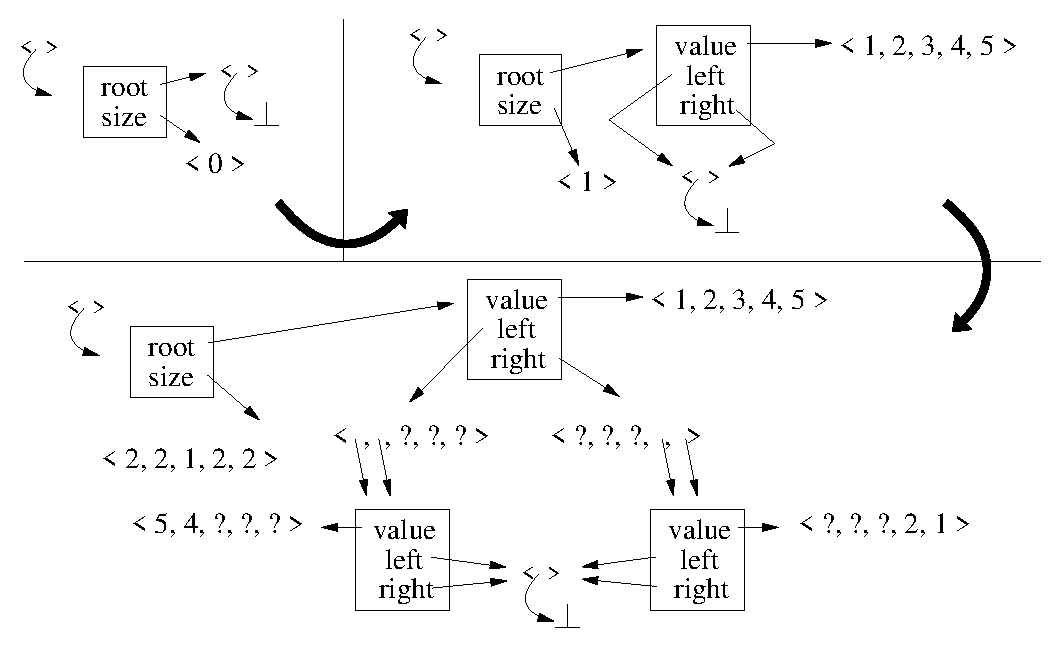
\includegraphics[scale=0.5]{figures/delta}
    }
    \caption{\label{fig:delta-state}Transition of delta states at the
      boundaries of method calls.}  
  \end{small}
\end{figure}
%%%%%%%%%%%% 

Consider, for illustration, that we want to execute the following
parameterized test sequence~\cite{tillmann05:parameterized} on inputs
(b,1,5), (b,2,4), (b,3,3), (b,4,2), and (b,5,1), where b holds a
reference to a newly created (empty) \CodeIn{BST} object.

{\small
\noindent
\begin{verbatim}
  //@ requires bst.size == 0
  void add2(BST bst, int a, int b) {
    /*1*/bst.add(a); /*2*/bst.add(b) /*3*/
  }
\end{verbatim}
}
\normalfont

\noindent
In standard mode we need to run the test for 5 times (once for each
input) to produce 5 distinct post-states of the tree.  In delta mode a
fewer number of executions are necessary.
Figure~\ref{fig:delta-state} shows the state of the tree(s) obtained
with the delta-mode execution of test sequence \CodeIn{add2} on input
(\lt{}b\gt{},\lt{}1,2,3,4,5\gt{},\lt{}5,4,3,2,1\gt{}).  We show
snaphots of the delta state associated with variable \CodeIn{bst} in
the positions marked 1,2, and 3 in \CodeIn{add2}.  We do not show
instrumented versions of the \CodeIn{BST} class and \CodeIn{add2} due
to space limitations.  We use braces to denote a set value, i.e., a
delta object.  We refer to a set with one single element as a
constant.  For example, all 5 individual states in this example refer
to the same tree object that variable \CodeIn{bst} refers to.  Similar
to a standard execution, the execution of the first call to
\CodeIn{add} sets the root node and increments the size of the tree.
The root node has field \CodeIn{value} set to \lt{}1,2,3,4,5\gt{} and
\CodeIn{left} and \CodeIn{right} fields set to the constant
\lt{}\CodeIn{null}\gt{}.  Unfortunately,\Comment{Unlike this first
  call to \CodeIn{add} however} sometimes it is not possible for every
individual state to ``agree'' with every control decision made during
the execution of one path.  In the second call to \CodeIn{add}, for
instance, \dE{} forks the execution at line 16 as only two individual
states evaluate the expression \CodeIn{tmp.info < info} to true.
Conceptually, the original sets \emph{splits} with this operations.
In practice, we use a state mask to indicate which individual states
are active in one execution path.  For this example, \DE{} traverses a
total of 3 paths (in 3 executions) until all 5 states from the input
set are explored.  At the bottom of the figure we show the final state
obtained after these three executions complete.

We list below the reasons for \dE{} speedups.

\mybull{Constants in the delta state.}  The cost of adding two
constant integer sets is comparable to the addition of two integers.
In scenarios where states are very similar these constants often
arise.  Important to note that some delta objects may become constants
after state masks are applied during execution.

\mybull{Fewer executions.}  \dE{} explores as many \emph{distinct}
paths as necessary.  For the example above, \DE{} explored 3 distinct
paths for the 5 input states.  Standard execution explored 2
additional paths to explore all states in the input set.  \dE{} can
save the duplicate cost of executing instructions that do not create
data.  For example, \CodeIn{PUSH}, \CodeIn{POP}, \CodeIn{INVOKE*},
etc.

Note that the performance of \DE{} depends on a number of factors.
One important factor is the number of splits necessary to cover all
states.  For example, previous results indicate that the delta
execution of \CodeIn{BST} performs worse than of a balanced tree.  The
number of nodes traversed in a given path of a balance tree is smaller
on average resulting in less
splits~\cite{damorim:issta2007,dAmorimLM08}.  One other factor is the
number of states and the similarity across them.  \DE{} works best
with many similar states.  In the context of mutation testing, we
assume that for large applications the number of mutations can be very
high.  In addition, the mutations will not dramatically modify the
state.

\Comment{
It is possible to partition the sets involved in an operation and
assign different threads to compute solutions for each
partition.\Comment{ Section~\ref{?}  shows that there will be no need
  of recombining solutions in a shared-memory programming model.}}

%% The initial goal of the technique was to speed up explicit-state model
%% checking.  \DE{} can take advantage of the control flow similarity
%% across different states to optimize time.  \DE{} can also take
%% advantage of data similarity for efficient data access: in the case
%% above, all four individual states share the \CodeIn{bst} object and
%% only one integer suffices to encode the size of all trees.  Very
%% important to note is that one execution in delta mode is expensive.
%% Split and merge, in particular, are costly operations.  Speedup
%% depends on a number of factors.  Specially, the number of states and
%% potential for sharing.

\subsection{Mutation Testing}
\label{sec:mut}

Mutation testing is a technique to assess the quality of a test suite.
The technique creates variants of the SUT, known as mutants.  Each
mutant represents potential errors that programmers could make.  The
technique evaluates the capability of the test suite to find such
errors.  The assumption is that a test suite that detects a high ratio
of artificial errors will have higher chances of detecting real
errors.  Mutation testing creates mutants by applying specific mutant
operators to the
code~\cite{offut-etal-1994,ma02:interclass,yu-seung-ma-etal-2005}.
For example, one possible mutant for the \CodeIn{BST} subject is
obtained by replacing the relational operator \CodeIn{>} at line 21
with \CodeIn{>=}.  Such small change has the effect of allowing
duplicate elements in the tree.  Several variants of this approach
have been proposed as to reduce analysis cost at the expense of
relaxing precision.  More specifically these variants often propose
weaker notions for mutation killing.  Examples include weak
mutation~\cite{howden82:weak}, second-order
mutation~\cite{macario-etal-2009}, and higher-order
mutation~\cite{jia-harman-2009}.  This paper focuses on strong
mutation.

\Comment{
Mutation testing assesses the quality of a test suite by inserting
artificial bugs into a program, and checking whether the test suite
finds them.  Mutation testing has two issues.  First, the \emph{time
  needed to check all mutations} --- the test suite has to be run for
every mutation. Second, the inability to automatically identify
\emph{equivalent mutations}, which are mutations that change the
syntax of the program but do not change its semantics.
}

\section{Approach: Combining Delta Execution and Mutation Testing}

A \emph{mutant schemata} is a variation of the SUT including all
generated mutants~\cite{millo-etal-1988}.  With the schemata, the
choice of which mutant to use in a test run is delayed to runtime.
Each mutation in the schemata is protected with a conditional that
checks whether or not the mutant is enabled for the execution.  The
schemata was originally proposed to reduce the high cost of compiling
mutants\Comment{ as only the mutant schemata requires compilation}; it
is also key to enable the application of \DE{} in mutation testing.
For the mutation example described in Section~\ref{sec:mut} the mutant
schemata will use the expression
\CodeIn{MUT\_GTE?temp.info>=info:temp.info>info} instead of
\CodeIn{temp.info>info}.  This indicates that the mutation will be
enabled if the user sets the flag \CodeIn{MUT\_GTE}.

We want \DE{} to execute all mutants for a given test
\emph{simultaneously}.  For that we run each test in delta mode using
the mutant schemata.  The delta execution will use $n + 1$ states,
where $n$ is the number of distinct mutants.  The additional state is
associated to the original program (no mutation).  At the point of
mutation \DE{} forks execution.  It performs a breadth-first
exploration of the paths associated to each branch.  In one execution
branch, the state set includes only the state id for the considered
mutant.  In the other branch, it considers all the other active
states.  Immediately after evaluating each branch, the states are
merged.  This avoids unnecessarily forking an additional execution to
explore the other state sets.  Without merging the states after
mutation points \DE{} would explore $k + 1$ paths, where $k$ is the
number of covered mutants.

For illustration, let's consider that the original program uses the
expression \CodeIn{x > y} and that the mutant schemata includes a
mutant for that expression that replaces \CodeIn{>} with \CodeIn{<}.
Additionally, consider that the mutant schemata contains 5 mutants and
the mutant above corresponds to mutant number 3.  \DE{} of one test on
the mutant schemata will have 6 individual states: 1 corresponding to
the original program and 5 for the mutants.  The evaluation of the
expression above on the mutant schemata with values \lt{}1\gt{} for
\CodeIn{x} and \lt{}2\gt{} for \CodeIn{y} results in
\lt{}f,f,f,t,f,f\gt{}.  Note the state at index 0 corresponds to the
original program.  Figure~\ref{fig:delta-schemata}...

%%%%%%%%%%%%  example test case
\subfiguretopcaptrue
\begin{figure}[t]
  \centering
  \begin{small}
    \subfigure{
      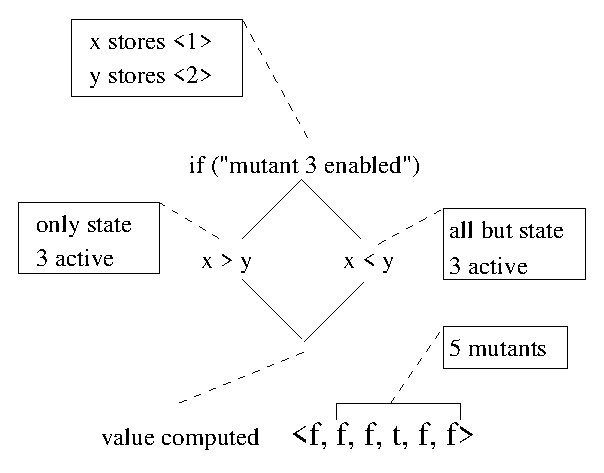
\includegraphics[scale=0.5]{figures/delta-schamata}
    }
    \caption{\label{fig:delta-schemata}Interpretation of mutated expression.}  
  \end{small}
\end{figure}
%%%%%%%%%%%% 

\subsection{Optimizations}

We list below general and mutation-specific optimizations of \DE{}.

\begin{itemize}

\item \textbf{Weak mutation} \DE{} ignores states from consideration
  when it covers a mutation with a test and that mutation does not
  affect state, i.e., that test does \emph{not} weakly kill the
  mutant.  In that case, the state becomes deactivated; no further
  operations will affect it.  The idea for this optimization is
  original from Fleyshgakker and Weiss
  work~\cite{FleyshgakkerWeiss-issta1994}.

\item \textbf{Native execution} The benefit of invoking a
  native-version delta operation (say, addition of two integer sets)
  conceptually increases with the number of elements in the sets.

\item \textbf{Enables parallel computation (novel).}  \DE{} can be
  parallelized in two ways.  It can delegate the computation of a
  value (say the addition of two sets) to a distinct thread.
  Execution blocks any thread that attempts to read from a not yet
  computed set.  Another way is to spawn a new thread to explore a new
  execution path at the split of a set.

\end{itemize}


\noindent\textbf{Speed up.}  Delta Execution can execute several
mutations in parallel.  However, speed ups depends on a number of
factors including the average number of covered mutations per test,
the potential for sharing data (and consequently control flow), and
average length of execution.  A one-state execution in delta mode is
slower than a standard execution.  A multi-state execution in delta
mode is likely slower if no sharing is observed or each execution
terminates very quickly.

%% \Comment{please check if this still makes sense. -M. PART1:Therefore,
%%   the state will be split for every mutation, as the mutated and
%%   unmutated code is executed on the current state.  A potential speed
%%   up are states that can be merged again, e.g the mutation did not
%%   affect the program state. Furthermore the execution that happens
%%   before a mutation does not have to be repeated for every mutation.
%%   PART2:How does delta execution deal with state derivations? E.g. a
%%   mutated execution takes different a control flow path than the
%%   normal execution.  PART 3:How would the split of states at mutations
%%   be implemented? --M paragraph still makes sense --DS}\\

\subsection{Implementation}

\Fix{...}

\section{Evaluation}

\Fix{...}

\section{Other applications}

This section discusses potential application of \DE{} within and
outside the context of mutation testing.

\vspace{1ex}\noindent\textbf{Measure Impact.}  The impact of a
mutation on state is helpful to improve a test
suite~\cite{schuler-issta-2009}.\Comment{please, let me know if there
  is other goal. -M} To that end, one can compare original and
individual state differences across one delta state.  We conjecture
that the higher the difference between non-mutated and mutated states
the higher the chance to observe the change with a test
execution.\Comment{don't understand this sentence.  thought that state
  change implies semantic changes. do you mean observable change?
  change in control flow? -M Yes, I meant an observable
  change. E.g. The program can have different state at some point but
  produces the same result, or only non-accessible values are changed
  that do not affect the result.-DS} Furthermore, the impact can
provide hints on how to improve the test suite. For example, one can
use information of state difference reachable from a test to augment
that test with state assertions.  \Comment{this is really nice! -M}

\vspace{1ex}\noindent\textbf{Detect equivalent executions.} \DE{}
expresses one state for each mutant plus one state for the original
program. It is therefore feasible to compare states, after the
activation of a mutation and at the end of a run. If there is no
difference between the states, this suggests that either the mutation
is equivalent or the input data was not chosen carefully enough.
\Comment{careful: I guess the mutation can be activated several
  times.}\Comment{i guess the former approach also has the same
  limitations.  the quality of daikon invariant is limited by the
  quality of operational profiles.}

\Comment{i guess we need to make sure the mutation is also
  unreachable. -M}

\Comment{I think it will not be feasible to prove that a mutation is
  equivalent since we only know that there is no state change for the
  input data provided by the test. There could exist other inputs that
  cause a state change.  However it might be a good indicator of
  equivalence. -D}

\Comment{i guess my comment was misplaced and confusing.  it was not
  about finding a mutant equivalent in the general case.  but in the
  case of a specific test.  that could help to optimize execution, not
  to rule out the mutant. -M}

\vspace{1ex}\noindent\textbf{Partition Mutations.}  \sloppy Similarity
of impact is a criteria to partition mutants: mutations that end up in
similar states, have similar effects in the program.  One can
conjecture that one test might detect all similar mutations or
none. This information is valuable to guide a programmer in the
improvement of a test suite.  He only needs to focus on one
representative of each partition.

\vspace{1ex}\noindent\textbf{Analysis of variation} \Fix{Software
  Product Lines...}


%% Weak mutation~\cite{brian-marick-1991,offut-etal-1994} is a more
%% efficient variant of the original (strong) mutation testing but offers
%% weaker guarantees.  In weak mutation it suffices for a test run to
%% observe state changes in the vicinity of the mutation point.  A
%% popular approach to cost reduction is to select minimum number of
%% operators to obtain nearly adequate full mutation coverage (as if all
%% operators were
%% selected)~\cite{millo-etal-1988,untch-offut-harrold-1993,offut-etal-1996}.
%% Schuler and Zeller~\cite{schuler-zeller-fse-2009,schuler-issta-2009}
%% save coverage data to avoid execution of tests that do not cover
%% mutants \Fix{...elaborate on equivalent mutant checking...}.  Jia and
%% Harman~\cite{jia-harman-2009} and Macario
%% \etal{}~\cite{macario-etal-2009} illustrate that higher order mutants
%% (i.e., a mutant that builds on other mutants) can significantly reduce
%% number of generated mutants at risk of killing just a few first-order
%% mutants.

%% ...~\cite{fleyshgakker-etal-1994}


%% A test $T$ \emph{strongly kills} a mutant $M$ if the outputs of
%% running $T$, respectively, on $P$ and $M$ differ.  A test $T$
%% \emph{kills weakly} mutant $M$ if running $T$ on $M$ produce state
%% changes with respect to $P$.  Weak mutation is a technique to reduce
%% cost of mutation testing~\cite{brian-marick-1991,offut-etal-1994}: a
%% test run terminates as soon as mutant is weakly killed (but without
%% assuring strongly killing).  A mutant can \emph{survive} mutation
%% testing if it is semantically \emph{equivalent} to the original
%% program or the test suite is inadequate.

%% The mutation testing approach produces a score proportional to the
%% number of mutants killed.  Conceptually, the higher such score the
%% better the suite (i.e, the fitter to find seeded faults).


%% Delta Execution (\de{}) is a technique initally proposed to speed up
%% the main operations involved in the model checking of programs with
%% heaps, namely, execution, backtracking, and state
%% comparison~\cite{dAmorimLM08}.  \de{} is a special mode of execution
%% that operates on set of states as opposed to one individual state.
%% The technique takes advantage of the similarity across the different
%% states in the set to speed up execution of a sequential program
%% block.\Comment{Conceptually, as long as control flow does not change
%%   across the execution of one instruction over each individual state
%%   in the set, \de{} can make a transition on a set of states as
%%   opposed to several transitions, each on one individual state.}  The
%% performance of our previous \de{} implementation related to a
%% significant extent to the presence of constants in these sets.  We
%% observed that, in the context of program model checking, these
%% constants often appear within sets.

%% Our goal is to scale delta execution, enabling it to operate on more
%% general scenarios~\cite{zhou-hotdep:2007}.  Our approach is to define
%% the main operations of \de{} in terms of Single Instruction Multiple
%% Data (SIMD) instructions available in modern CPU processors.
%% Conceptually, a SIMD instruction operates against input vector
%% arguments; processor units execute in parallel the same operation on
%% each vector element.  This paper illustrates how \de{} leverages these
%% SIMD instructions to speed up Multiple Almost Redundant Executions
%% (MARE).  We show that with this modification we can significantly
%% speed up mutation testing, a special case of MARE.

%% The contributions of this work are as follows:
%% \begin{itemize}
%% \item \textbf{Idea}
%% \item \textbf{Evaluation}
%% \item \textbf{Implementation}
%% \end{itemize}

%% \section{Example}

%% \section{Evaluation}

%% \subsection{Speed up bounded-exhaustive testing}

%% \subsection{Speed up mutation testing}


\section{Related Work}

Researchers have proposed several optimizations to speed up mutation
analysis.  For example, Marick~\etal~\cite{brian-marick-1991} propose
a variant of original (strong) mutation testing known as weak
mutation.  In this variant the decision on whether execution of the
mutant behaves differently is anticipated to the vicinity of the code
change; hence speeding up test execution at the expense of weakening
correctness guarantees.  Untch~\etal{}~\cite{untch-offut-harrold-1993}
combine all mutants in a single program known as mutant schemata to
save mutant compilation costs.  This approach is used in more recent
implementations such as Mu-Java~\cite{yu-seung-ma-etal-2005} and
Javalanche~\cite{schuler-zeller-fse-2009}.  Another popular approach
to cost reduction is to select minimum number of operators that will
be almost as
effective~\cite{millo-etal-1988,untch-offut-harrold-1993,offut-etal-1996,schuler-issta-2009}.
Finally yet another optimization is to re-execute a test for a mutant
only if that test is known to cover that
mutant~\cite{schuler-zeller-fse-2009}.  The mutant schemata enables
efficient finding of such covered mutants.

Researchers have also proposed approaches to detect likely equivalent
mutants.  \Fix{...}

\Comment{
Another problem in mutation testing is the lack of automated support
to the analysis of live mutants. \Fix{...}
}

\section{Conclusions}

\Fix{Future work.  Partitioning...}

\bibliographystyle{IEEEtranBST/IEEEtran}
\bibliography{testing}
%%\bibliography{short-description-testing}

\end{document}

